\section[Breve reseña histórica]{Breve reseña histórica de la utilización de las
    \gls{tic} en la educación}

El análisis de la historia de las \Gls{tic} en educación es
indispensable\cite{mcdougall2006theory}. Existe una corriente que tiende a
desestimar las experiencias pasadas, cuyo principal fundamento es la velocidad
con la que la tecnología evoluciona, es importante el estudio de la evolución de
la misma pues los errores pedagógicos cometidos, aunque puedan parecer evidentes
hoy en día, condujeron a nuevos modelos y conclusiones que son la base de la
utilización de las \Gls{tic} actualmente\cite{mcdougall2006theory}. Así, el uso
de las \Gls{tic} en la educación no ha sido constante durante su historia, sino
más bien, ha evolucionado de ser un medio más de traspaso de información, hasta
hoy en día, donde permite construir conocimiento\cite{tinio:ict}.

La historia de las \Gls{tic} en educación comienza en la \enquote{Open
    University of United Kingdom} que en $1969$ se establece como la primera
institución educativa dedicada a la enseñanza a distancia utilizando las, para
aquel entonces, nuevas tecnologías\cite{tinio:ict}.

Para entender la historia de las \Gls{tic} en la educación, se presenta la
figura~\ref{fig:history_tics}, en la cual se observa la evolución que sufrió la
utilización de las \Gls{tic} como herramienta educativa. 

\begin{figure}[h]
\centering
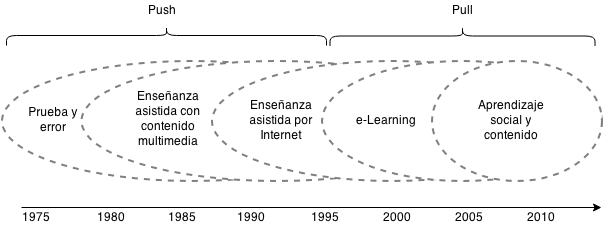
\includegraphics[scale=0.75]{tics/images/tics_history.png}
\caption{Utilización de las \Gls{tic} en la educación desde el año $1975$. Las
    fechas utilizadas son relacionadas a la evolución en los Estados Unidos de
    Norte America.}
\label{fig:history_tics}
\end{figure}



%Se observa que se
%parte la historia en cinco corrientes definidas, y a la vez, estas corrientes se
%agrupan según el mecanismo de traspaso de información, las tres primeras
%corrientes se denominan \textit{push} y las siguientes dos se denominan
%\textit{pull}. 

Se observan dos metodologías de traspaso de la información, \textit{push}, y
\textit{pull}. En el modelo \textit{push} los estudiantes obtienen información
sin una participación activa en la creación de esa información\cite{white:ict}.
La corrientes pedagógicas que marcan tendencia en este modelo son el
instruccionismo y el conductismo\cite{white:ict,leinonen:ict}. Las fases que se
observan en la figura~\ref{fig:history_tics} durante el periodo \textit{push},
son la utilización de ejercicios de prueba y error sistemáticos, y la
distribución de contenido educativo primeramente a través de discos ópticos, y
luego a través de Internet\cite{leinonen:ict}.

La evolución de la tecnología permite mejorar los mecanismos de comunicación,
creando redes interactivas donde se comparte la información, así se inicia el
modelo \textit{pull}, en él, los alumnos son creadores activos de
conocimiento\cite{white:ict,leinonen:ict}. Se intensifica la creación de
herramientas basadas en el constructivismo y el construccionismo. Ejemplos de
las tecnologías en este período son el \textit{e-Learning}, y plataformas de
interacción social como wikis, blogs, y otros\cite{leinonen:ict}.

En la figura~\ref{fig:history_tics} se observa el solapamiento entre los
diversos mecanismos utilizados. Se muestra el inicio de la utilización de una
herramienta, pero no su fin, actualmente se siguen utilizando todas las
tecnologías y modelos\cite{leinonen:ict}.

Aunque la figura~\ref{fig:history_tics} muestre un progreso lineal de las
corrientes, este progreso no es igual en todo el mundo, y el grado de impacto de
las \Gls{tic} varia entre países, lo que se conoce como \enquote{brecha
    tecnológica}.

